\documentclass[twoside]{book}

% Packages required by doxygen
\usepackage{fixltx2e}
\usepackage{calc}
\usepackage{doxygen}
\usepackage[export]{adjustbox} % also loads graphicx
\usepackage{graphicx}
\usepackage[utf8]{inputenc}
\usepackage{makeidx}
\usepackage{multicol}
\usepackage{multirow}
\PassOptionsToPackage{warn}{textcomp}
\usepackage{textcomp}
\usepackage[nointegrals]{wasysym}
\usepackage[table]{xcolor}

% Font selection
\usepackage[T1]{fontenc}
\usepackage[scaled=.90]{helvet}
\usepackage{courier}
\usepackage{amssymb}
\usepackage{sectsty}
\renewcommand{\familydefault}{\sfdefault}
\allsectionsfont{%
  \fontseries{bc}\selectfont%
  \color{darkgray}%
}
\renewcommand{\DoxyLabelFont}{%
  \fontseries{bc}\selectfont%
  \color{darkgray}%
}
\newcommand{\+}{\discretionary{\mbox{\scriptsize$\hookleftarrow$}}{}{}}

% Page & text layout
\usepackage{geometry}
\geometry{%
  a4paper,%
  top=2.5cm,%
  bottom=2.5cm,%
  left=2.5cm,%
  right=2.5cm%
}
\tolerance=750
\hfuzz=15pt
\hbadness=750
\setlength{\emergencystretch}{15pt}
\setlength{\parindent}{0cm}
\setlength{\parskip}{3ex plus 2ex minus 2ex}
\makeatletter
\renewcommand{\paragraph}{%
  \@startsection{paragraph}{4}{0ex}{-1.0ex}{1.0ex}{%
    \normalfont\normalsize\bfseries\SS@parafont%
  }%
}
\renewcommand{\subparagraph}{%
  \@startsection{subparagraph}{5}{0ex}{-1.0ex}{1.0ex}{%
    \normalfont\normalsize\bfseries\SS@subparafont%
  }%
}
\makeatother

% Headers & footers
\usepackage{fancyhdr}
\pagestyle{fancyplain}
\fancyhead[LE]{\fancyplain{}{\bfseries\thepage}}
\fancyhead[CE]{\fancyplain{}{}}
\fancyhead[RE]{\fancyplain{}{\bfseries\leftmark}}
\fancyhead[LO]{\fancyplain{}{\bfseries\rightmark}}
\fancyhead[CO]{\fancyplain{}{}}
\fancyhead[RO]{\fancyplain{}{\bfseries\thepage}}
\fancyfoot[LE]{\fancyplain{}{}}
\fancyfoot[CE]{\fancyplain{}{}}
\fancyfoot[RE]{\fancyplain{}{\bfseries\scriptsize Generated by Doxygen }}
\fancyfoot[LO]{\fancyplain{}{\bfseries\scriptsize Generated by Doxygen }}
\fancyfoot[CO]{\fancyplain{}{}}
\fancyfoot[RO]{\fancyplain{}{}}
\renewcommand{\footrulewidth}{0.4pt}
\renewcommand{\chaptermark}[1]{%
  \markboth{#1}{}%
}
\renewcommand{\sectionmark}[1]{%
  \markright{\thesection\ #1}%
}

% Indices & bibliography
\usepackage{natbib}
\usepackage[titles]{tocloft}
\setcounter{tocdepth}{3}
\setcounter{secnumdepth}{5}
\makeindex

% Hyperlinks (required, but should be loaded last)
\usepackage{ifpdf}
\ifpdf
  \usepackage[pdftex,pagebackref=true]{hyperref}
\else
  \usepackage[ps2pdf,pagebackref=true]{hyperref}
\fi
\hypersetup{%
  colorlinks=true,%
  linkcolor=blue,%
  citecolor=blue,%
  unicode%
}

% Custom commands
\newcommand{\clearemptydoublepage}{%
  \newpage{\pagestyle{empty}\cleardoublepage}%
}

\usepackage{caption}
\captionsetup{labelsep=space,justification=centering,font={bf},singlelinecheck=off,skip=4pt,position=top}

%===== C O N T E N T S =====

\begin{document}

% Titlepage & ToC
\hypersetup{pageanchor=false,
             bookmarksnumbered=true,
             pdfencoding=unicode
            }
\pagenumbering{roman}
\begin{titlepage}
\vspace*{7cm}
\begin{center}%
{\Large My Project }\\
\vspace*{1cm}
{\large Generated by Doxygen 1.8.11}\\
\end{center}
\end{titlepage}
\clearemptydoublepage
\tableofcontents
\clearemptydoublepage
\pagenumbering{arabic}
\hypersetup{pageanchor=true}

%--- Begin generated contents ---
\chapter{Hierarchical Index}
\section{Class Hierarchy}
This inheritance list is sorted roughly, but not completely, alphabetically\+:\begin{DoxyCompactList}
\item Mono\+Behaviour\begin{DoxyCompactList}
\item \contentsline{section}{Fading}{\pageref{class_fading}}{}
\item \contentsline{section}{Gaze\+Over}{\pageref{class_gaze_over}}{}
\item \contentsline{section}{Spawn\+Selected\+Level}{\pageref{class_spawn_selected_level}}{}
\item \contentsline{section}{Torus}{\pageref{class_torus}}{}
\item \contentsline{section}{Torus\+Generator}{\pageref{class_torus_generator}}{}
\end{DoxyCompactList}
\end{DoxyCompactList}

\chapter{Class Index}
\section{Class List}
Here are the classes, structs, unions and interfaces with brief descriptions\+:\begin{DoxyCompactList}
\item\contentsline{section}{\hyperlink{class_connect_and_create_tower_manager}{Connect\+And\+Create\+Tower\+Manager} }{\pageref{class_connect_and_create_tower_manager}}{}
\item\contentsline{section}{\hyperlink{class_connect_and_join_test}{Connect\+And\+Join\+Test} }{\pageref{class_connect_and_join_test}}{}
\item\contentsline{section}{\hyperlink{class_create_new_game}{Create\+New\+Game} }{\pageref{class_create_new_game}}{}
\item\contentsline{section}{\hyperlink{class_fading}{Fading} }{\pageref{class_fading}}{}
\item\contentsline{section}{\hyperlink{class_f_p_s_display}{F\+P\+S\+Display} }{\pageref{class_f_p_s_display}}{}
\item\contentsline{section}{\hyperlink{class_tower_v_r_1_1_game_state}{Tower\+V\+R.\+Game\+State} }{\pageref{class_tower_v_r_1_1_game_state}}{}
\item\contentsline{section}{\hyperlink{class_tower_v_r_1_1_game_state_changed_event}{Tower\+V\+R.\+Game\+State\+Changed\+Event} }{\pageref{class_tower_v_r_1_1_game_state_changed_event}}{}
\item\contentsline{section}{\hyperlink{class_gaze_over}{Gaze\+Over} }{\pageref{class_gaze_over}}{}
\item\contentsline{section}{\hyperlink{interface_tower_v_r_1_1_i_tower_game_manager}{Tower\+V\+R.\+I\+Tower\+Game\+Manager} }{\pageref{interface_tower_v_r_1_1_i_tower_game_manager}}{}
\item\contentsline{section}{\hyperlink{class_join_server}{Join\+Server} }{\pageref{class_join_server}}{}
\item\contentsline{section}{\hyperlink{class_vuforia_1_1_lost_tracking}{Vuforia.\+Lost\+Tracking} }{\pageref{class_vuforia_1_1_lost_tracking}}{}
\item\contentsline{section}{\hyperlink{class_master_client_only_behaviour}{Master\+Client\+Only\+Behaviour} }{\pageref{class_master_client_only_behaviour}}{}
\item\contentsline{section}{\hyperlink{class_tower_v_r_1_1_master_client_only_behaviour}{Tower\+V\+R.\+Master\+Client\+Only\+Behaviour} }{\pageref{class_tower_v_r_1_1_master_client_only_behaviour}}{}
\item\contentsline{section}{\hyperlink{class_tower_v_r_1_1_master_start_game}{Tower\+V\+R.\+Master\+Start\+Game} }{\pageref{class_tower_v_r_1_1_master_start_game}}{}
\item\contentsline{section}{\hyperlink{class_tower_v_r_1_1_master_tower_game_manager_impl}{Tower\+V\+R.\+Master\+Tower\+Game\+Manager\+Impl} }{\pageref{class_tower_v_r_1_1_master_tower_game_manager_impl}}{}
\item\contentsline{section}{\hyperlink{class_networked_behaviour}{Networked\+Behaviour} }{\pageref{class_networked_behaviour}}{}
\item\contentsline{section}{\hyperlink{class_tower_v_r_1_1_network_event_codes}{Tower\+V\+R.\+Network\+Event\+Codes} }{\pageref{class_tower_v_r_1_1_network_event_codes}}{}
\item\contentsline{section}{\hyperlink{class_tower_v_r_1_1_next_player_event}{Tower\+V\+R.\+Next\+Player\+Event} }{\pageref{class_tower_v_r_1_1_next_player_event}}{}
\item\contentsline{section}{\hyperlink{class_photon_network_event}{Photon\+Network\+Event} }{\pageref{class_photon_network_event}}{}
\item\contentsline{section}{\hyperlink{class_tower_v_r_1_1_place_tower_piece_event}{Tower\+V\+R.\+Place\+Tower\+Piece\+Event} }{\pageref{class_tower_v_r_1_1_place_tower_piece_event}}{}
\item\contentsline{section}{\hyperlink{class_player_camera_movement}{Player\+Camera\+Movement} }{\pageref{class_player_camera_movement}}{}
\item\contentsline{section}{\hyperlink{class_tower_v_r_1_1_player_lost_event}{Tower\+V\+R.\+Player\+Lost\+Event} }{\pageref{class_tower_v_r_1_1_player_lost_event}}{}
\item\contentsline{section}{\hyperlink{class_tower_v_r_1_1_player_ready_event}{Tower\+V\+R.\+Player\+Ready\+Event} }{\pageref{class_tower_v_r_1_1_player_ready_event}}{}
\item\contentsline{section}{\hyperlink{class_tower_v_r_1_1_player_turn_observer}{Tower\+V\+R.\+Player\+Turn\+Observer} }{\pageref{class_tower_v_r_1_1_player_turn_observer}}{}
\item\contentsline{section}{\hyperlink{class_tower_v_r_1_1_player_won_event}{Tower\+V\+R.\+Player\+Won\+Event} }{\pageref{class_tower_v_r_1_1_player_won_event}}{}
\item\contentsline{section}{\hyperlink{class_randomize_server_name}{Randomize\+Server\+Name} }{\pageref{class_randomize_server_name}}{}
\item\contentsline{section}{\hyperlink{classremove_target_child}{remove\+Target\+Child} }{\pageref{classremove_target_child}}{}
\item\contentsline{section}{\hyperlink{class_restrict_to_host}{Restrict\+To\+Host} }{\pageref{class_restrict_to_host}}{}
\item\contentsline{section}{\hyperlink{class_retrieve_and_spawn_players}{Retrieve\+And\+Spawn\+Players} }{\pageref{class_retrieve_and_spawn_players}}{}
\item\contentsline{section}{\hyperlink{class_scene_transition_manager}{Scene\+Transition\+Manager$<$ T $>$} }{\pageref{class_scene_transition_manager}}{}
\item\contentsline{section}{\hyperlink{struct_tower_v_r_1_1_score}{Tower\+V\+R.\+Score} }{\pageref{struct_tower_v_r_1_1_score}}{}
\item\contentsline{section}{\hyperlink{class_tower_v_r_1_1_score_changed_event}{Tower\+V\+R.\+Score\+Changed\+Event} }{\pageref{class_tower_v_r_1_1_score_changed_event}}{}
\item\contentsline{section}{\hyperlink{class_tower_v_r_1_1_select_tower_piece_event}{Tower\+V\+R.\+Select\+Tower\+Piece\+Event} }{\pageref{class_tower_v_r_1_1_select_tower_piece_event}}{}
\item\contentsline{section}{\hyperlink{class_set_max_players}{Set\+Max\+Players} }{\pageref{class_set_max_players}}{}
\item\contentsline{section}{\hyperlink{class_show_servers}{Show\+Servers} }{\pageref{class_show_servers}}{}
\item\contentsline{section}{\hyperlink{class_singleton}{Singleton$<$ T $>$} }{\pageref{class_singleton}}{}
\item\contentsline{section}{\hyperlink{class_spawn_selected_level}{Spawn\+Selected\+Level} }{\pageref{class_spawn_selected_level}}{}
\item\contentsline{section}{\hyperlink{class_timer}{Timer} }{\pageref{class_timer}}{}
\item\contentsline{section}{\hyperlink{class_torus}{Torus} }{\pageref{class_torus}}{}
\item\contentsline{section}{\hyperlink{class_torus_generator}{Torus\+Generator} }{\pageref{class_torus_generator}}{}
\item\contentsline{section}{\hyperlink{class_tower_v_r_1_1_tower_game_behaviour}{Tower\+V\+R.\+Tower\+Game\+Behaviour} }{\pageref{class_tower_v_r_1_1_tower_game_behaviour}}{}
\item\contentsline{section}{\hyperlink{class_tower_v_r_1_1_tower_game_manager}{Tower\+V\+R.\+Tower\+Game\+Manager} }{\pageref{class_tower_v_r_1_1_tower_game_manager}}{}
\item\contentsline{section}{\hyperlink{class_tower_v_r_1_1_tower_game_manager_impl}{Tower\+V\+R.\+Tower\+Game\+Manager\+Impl} }{\pageref{class_tower_v_r_1_1_tower_game_manager_impl}}{}
\item\contentsline{section}{\hyperlink{class_tower_v_r_1_1_tower_piece}{Tower\+V\+R.\+Tower\+Piece} }{\pageref{class_tower_v_r_1_1_tower_piece}}{}
\item\contentsline{section}{\hyperlink{class_tower_v_r_1_1_tower_piece_info}{Tower\+V\+R.\+Tower\+Piece\+Info} }{\pageref{class_tower_v_r_1_1_tower_piece_info}}{}
\item\contentsline{section}{\hyperlink{class_tower_v_r_1_1_tower_piece_spawner}{Tower\+V\+R.\+Tower\+Piece\+Spawner} }{\pageref{class_tower_v_r_1_1_tower_piece_spawner}}{}
\item\contentsline{section}{\hyperlink{class_transform_debugger}{Transform\+Debugger} }{\pageref{class_transform_debugger}}{}
\item\contentsline{section}{\hyperlink{class_tower_v_r_1_1_try_start_game_event}{Tower\+V\+R.\+Try\+Start\+Game\+Event} }{\pageref{class_tower_v_r_1_1_try_start_game_event}}{}
\item\contentsline{section}{\hyperlink{class_tower_v_r_1_1_turn_state}{Tower\+V\+R.\+Turn\+State} }{\pageref{class_tower_v_r_1_1_turn_state}}{}
\item\contentsline{section}{\hyperlink{class_tower_v_r_1_1_turn_state_changed_event}{Tower\+V\+R.\+Turn\+State\+Changed\+Event} }{\pageref{class_tower_v_r_1_1_turn_state_changed_event}}{}
\item\contentsline{section}{\hyperlink{class_tower_v_r_1_1_turn_time_limits}{Tower\+V\+R.\+Turn\+Time\+Limits} }{\pageref{class_tower_v_r_1_1_turn_time_limits}}{}
\end{DoxyCompactList}

\chapter{Class Documentation}
\hypertarget{class_fading}{}\section{Fading Class Reference}
\label{class_fading}\index{Fading@{Fading}}
Inheritance diagram for Fading\+:\begin{figure}[H]
\begin{center}
\leavevmode
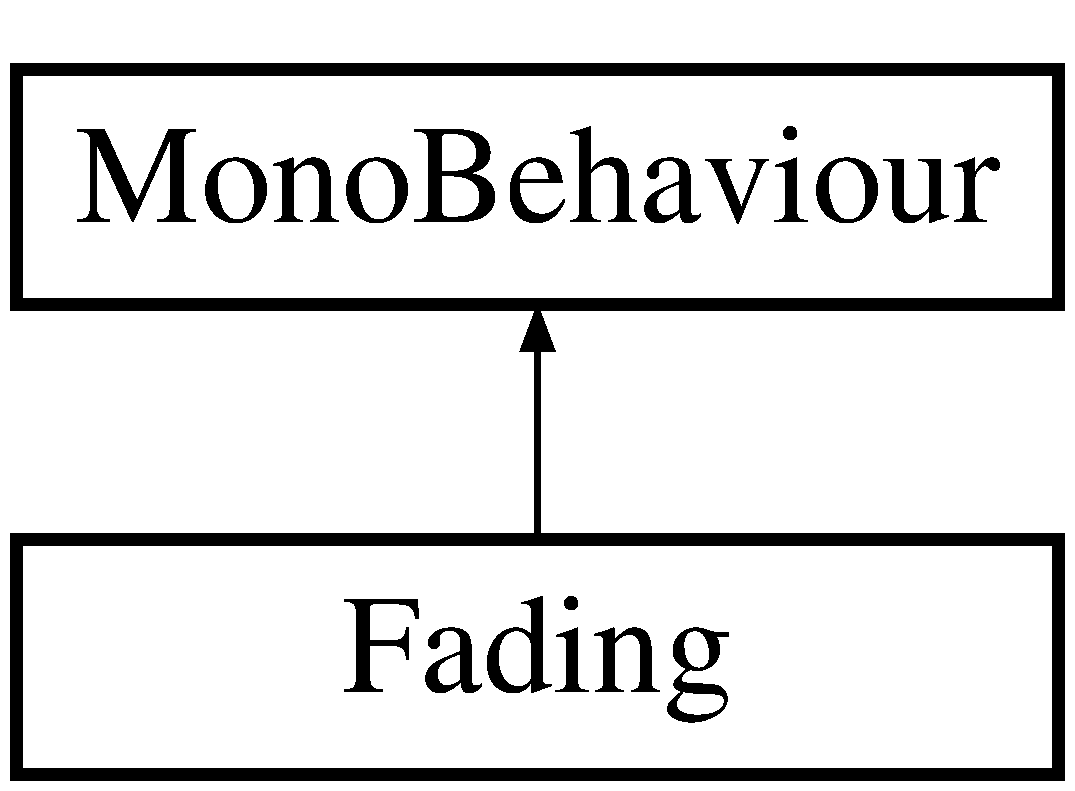
\includegraphics[height=2.000000cm]{class_fading}
\end{center}
\end{figure}
\subsection*{Public Member Functions}
\begin{DoxyCompactItemize}
\item 
float {\bfseries Begin\+Fade} (int direction)\hypertarget{class_fading_aad79c9805adb309dfca9c35956a6539f}{}\label{class_fading_aad79c9805adb309dfca9c35956a6539f}

\end{DoxyCompactItemize}
\subsection*{Public Attributes}
\begin{DoxyCompactItemize}
\item 
Texture2D {\bfseries fade\+Out\+Texture}\hypertarget{class_fading_aaba5de61bbf5cd88b53a8d2b81f074a1}{}\label{class_fading_aaba5de61bbf5cd88b53a8d2b81f074a1}

\item 
float {\bfseries fade\+Speed} = 0.\+0f\hypertarget{class_fading_a4850e50beaca24d0a3266221a36f1e5a}{}\label{class_fading_a4850e50beaca24d0a3266221a36f1e5a}

\end{DoxyCompactItemize}


The documentation for this class was generated from the following file\+:\begin{DoxyCompactItemize}
\item 
/\+Users/benjamin/\+Programmering/\+Android\+H\+M\+D/\+Tower\+V\+R/\+Assets/\+Scripts/\+Custom/Fading.\+cs\end{DoxyCompactItemize}

\hypertarget{class_gaze_over}{}\section{Gaze\+Over Class Reference}
\label{class_gaze_over}\index{Gaze\+Over@{Gaze\+Over}}
Inheritance diagram for Gaze\+Over\+:\begin{figure}[H]
\begin{center}
\leavevmode
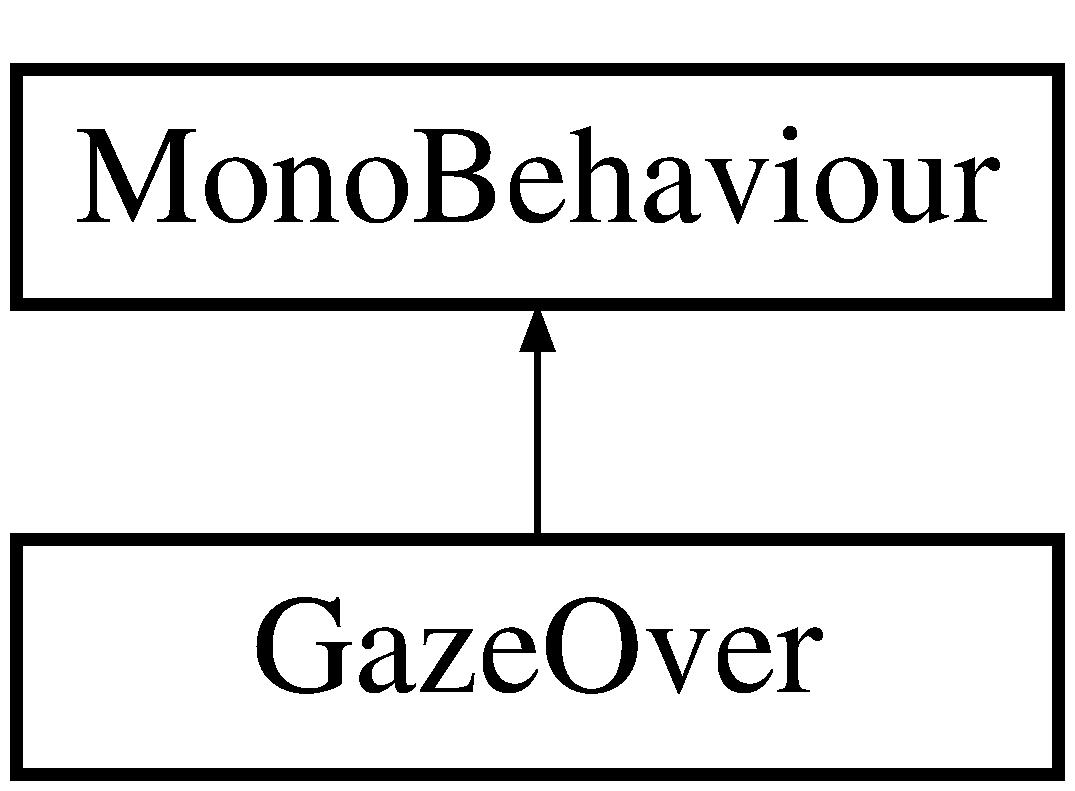
\includegraphics[height=2.000000cm]{class_gaze_over}
\end{center}
\end{figure}
\subsection*{Public Member Functions}
\begin{DoxyCompactItemize}
\item 
void {\bfseries Switch\+Scene} ()\hypertarget{class_gaze_over_a3bb891d7e1c1baf91593d2d975c98ef1}{}\label{class_gaze_over_a3bb891d7e1c1baf91593d2d975c98ef1}

\item 
void {\bfseries Load\+Scene} ()\hypertarget{class_gaze_over_a81b841907b39b75f68a04fef02a5923d}{}\label{class_gaze_over_a81b841907b39b75f68a04fef02a5923d}

\item 
void {\bfseries On\+Pointer\+Enter} ()\hypertarget{class_gaze_over_a8542b157da5e6c98d4500fa96b34e169}{}\label{class_gaze_over_a8542b157da5e6c98d4500fa96b34e169}

\item 
void {\bfseries On\+Pointer\+Exit} ()\hypertarget{class_gaze_over_ac6babe5ebb9a2fe681d559ab64b4f4ad}{}\label{class_gaze_over_ac6babe5ebb9a2fe681d559ab64b4f4ad}

\end{DoxyCompactItemize}
\subsection*{Public Attributes}
\begin{DoxyCompactItemize}
\item 
bool {\bfseries load\+Scene\+For\+All\+Players} = false\hypertarget{class_gaze_over_a1f3d93693093000a182971f54abea678}{}\label{class_gaze_over_a1f3d93693093000a182971f54abea678}

\item 
int {\bfseries level\+Index}\hypertarget{class_gaze_over_a4da14b1f14785e43084c6f5adeb7e641}{}\label{class_gaze_over_a4da14b1f14785e43084c6f5adeb7e641}

\item 
string {\bfseries Level\+Name}\hypertarget{class_gaze_over_a737fc0bbf32691a235d632475daab772}{}\label{class_gaze_over_a737fc0bbf32691a235d632475daab772}

\item 
string {\bfseries Level\+Material1}\hypertarget{class_gaze_over_abaa5c39e1a53eeda5e00a1727da499c6}{}\label{class_gaze_over_abaa5c39e1a53eeda5e00a1727da499c6}

\item 
string {\bfseries Level\+Skybox}\hypertarget{class_gaze_over_ae0fffd931b90309c155a73342ab4c50f}{}\label{class_gaze_over_ae0fffd931b90309c155a73342ab4c50f}

\end{DoxyCompactItemize}


\subsection{Detailed Description}
A class for switching scenes. How to use\+: Make sure your object has a Collider. Add this script and set which scene it should chnage to with index (from build settings). Add Event\+Trigger-\/component and use Pointer Down, Pointer Enter, Pointer Exit for the functions below. Check the box for the load\+Scene\+For\+All\+Players variable to use Photons functionality to sync the loaded scene. 

The documentation for this class was generated from the following file\+:\begin{DoxyCompactItemize}
\item 
/\+Users/benjamin/\+Programmering/\+Android\+H\+M\+D/\+Tower\+V\+R/\+Assets/\+Scripts/\+Custom/Gaze\+Over.\+cs\end{DoxyCompactItemize}

\hypertarget{class_spawn_selected_level}{}\section{Spawn\+Selected\+Level Class Reference}
\label{class_spawn_selected_level}\index{Spawn\+Selected\+Level@{Spawn\+Selected\+Level}}
Inheritance diagram for Spawn\+Selected\+Level\+:\begin{figure}[H]
\begin{center}
\leavevmode
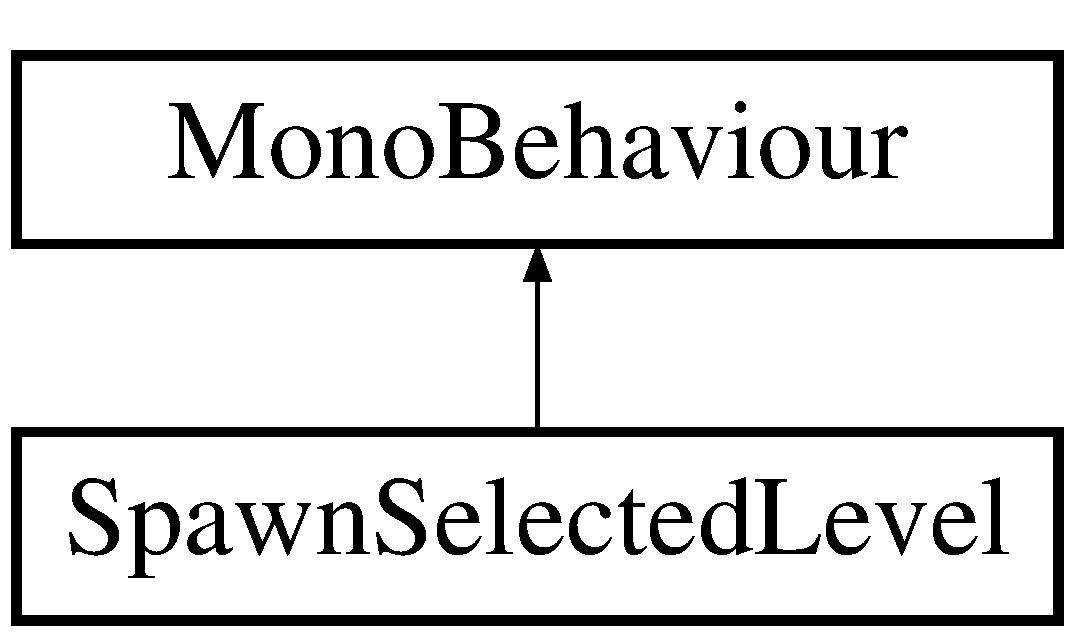
\includegraphics[height=2.000000cm]{class_spawn_selected_level}
\end{center}
\end{figure}
\subsection*{Public Attributes}
\begin{DoxyCompactItemize}
\item 
Game\+Object {\bfseries Level\+Components}\hypertarget{class_spawn_selected_level_a604f58d67bb353137f526689fecd1738}{}\label{class_spawn_selected_level_a604f58d67bb353137f526689fecd1738}

\item 
Material {\bfseries Material1}\hypertarget{class_spawn_selected_level_a366848fc78a8c064b11ca751d3d6025a}{}\label{class_spawn_selected_level_a366848fc78a8c064b11ca751d3d6025a}

\item 
Material {\bfseries Skybox}\hypertarget{class_spawn_selected_level_a13d055e319c08c9e52f37d8b810889f0}{}\label{class_spawn_selected_level_a13d055e319c08c9e52f37d8b810889f0}

\end{DoxyCompactItemize}
\subsection*{Static Public Attributes}
\begin{DoxyCompactItemize}
\item 
static string \hyperlink{class_spawn_selected_level_a8d218aa712c1464b1e6a928e52cdb56f}{Loaded\+Level}
\item 
static string {\bfseries Loaded\+Material1}\hypertarget{class_spawn_selected_level_a47b76272906237a6f5eb652908cebda6}{}\label{class_spawn_selected_level_a47b76272906237a6f5eb652908cebda6}

\item 
static string {\bfseries Loaded\+Skybox}\hypertarget{class_spawn_selected_level_a572973e025315254b42897c1bf2d5f3e}{}\label{class_spawn_selected_level_a572973e025315254b42897c1bf2d5f3e}

\end{DoxyCompactItemize}


\subsection{Member Data Documentation}
\index{Spawn\+Selected\+Level@{Spawn\+Selected\+Level}!Loaded\+Level@{Loaded\+Level}}
\index{Loaded\+Level@{Loaded\+Level}!Spawn\+Selected\+Level@{Spawn\+Selected\+Level}}
\subsubsection[{\texorpdfstring{Loaded\+Level}{LoadedLevel}}]{\setlength{\rightskip}{0pt plus 5cm}string Spawn\+Selected\+Level.\+Loaded\+Level\hspace{0.3cm}{\ttfamily [static]}}\hypertarget{class_spawn_selected_level_a8d218aa712c1464b1e6a928e52cdb56f}{}\label{class_spawn_selected_level_a8d218aa712c1464b1e6a928e52cdb56f}
Assume the level selection scene is \char`\"{}\+Scene 0\char`\"{} and the game scene is \char`\"{}\+Scene 1\char`\"{}.

Add this script to the scene manager in the game scene. (Scene 1) This scripts needs info form another script on the level-\/selection object ( in Scene 0). The public static string variables in this scripts should be assigned when clicking the level-\/selection object (in another script in scene 0). -\/\+EX\+: On\+Click()\{\hyperlink{class_spawn_selected_level_a8d218aa712c1464b1e6a928e52cdb56f}{Spawn\+Selected\+Level.\+Loaded\+Level} = Level\+Name;\} //\+When clicking (selecting the level), set the name of the prefab level to load.

See example in the script \char`\"{}\+Mouse\+Over.\+cs\char`\"{} in the Unity/\+Scripts folder (Google Drive).

O\+BS\+: Remember to destroy objects when leaving the scene. 

The documentation for this class was generated from the following file\+:\begin{DoxyCompactItemize}
\item 
/\+Users/benjamin/\+Programmering/\+Android\+H\+M\+D/\+Tower\+V\+R/\+Assets/\+Scripts/\+Custom/Spawn\+Selected\+Level.\+cs\end{DoxyCompactItemize}

\hypertarget{class_torus}{}\section{Torus Class Reference}
\label{class_torus}\index{Torus@{Torus}}
Inheritance diagram for Torus\+:\begin{figure}[H]
\begin{center}
\leavevmode
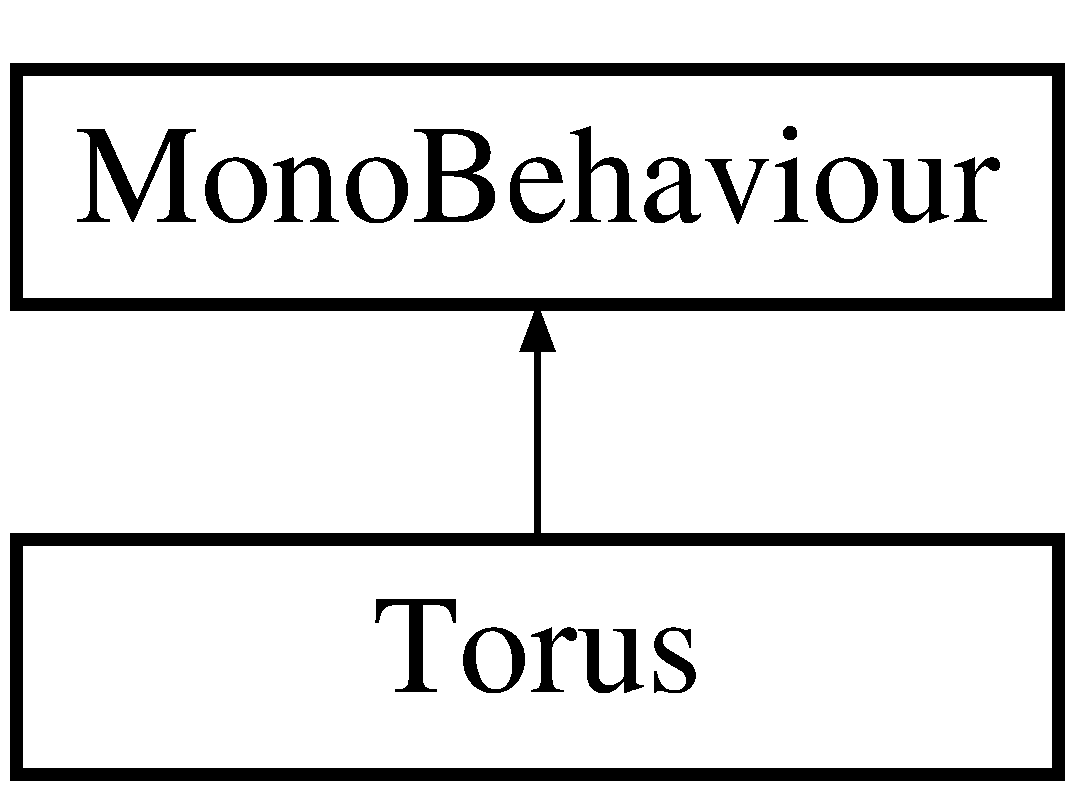
\includegraphics[height=2.000000cm]{class_torus}
\end{center}
\end{figure}
\subsection*{Public Member Functions}
\begin{DoxyCompactItemize}
\item 
void {\bfseries Refresh\+Torus} ()\hypertarget{class_torus_a11488676c74af823a124085c3af72aa3}{}\label{class_torus_a11488676c74af823a124085c3af72aa3}

\end{DoxyCompactItemize}
\subsection*{Public Attributes}
\begin{DoxyCompactItemize}
\item 
float {\bfseries segment\+Radius} = 1f\hypertarget{class_torus_a8dd1e53cd1fb9415fbe64b7004ba274c}{}\label{class_torus_a8dd1e53cd1fb9415fbe64b7004ba274c}

\item 
float {\bfseries tube\+Radius} = 0.\+1f\hypertarget{class_torus_af176474a9c7b704f10c2fd58b33771f8}{}\label{class_torus_af176474a9c7b704f10c2fd58b33771f8}

\item 
int {\bfseries num\+Segments} = 32\hypertarget{class_torus_a5c0c35544de72aa99edaa76d5b7357d8}{}\label{class_torus_a5c0c35544de72aa99edaa76d5b7357d8}

\item 
int {\bfseries num\+Tubes} = 12\hypertarget{class_torus_a7f981e7fbdfedb7170aba45013673dff}{}\label{class_torus_a7f981e7fbdfedb7170aba45013673dff}

\end{DoxyCompactItemize}


The documentation for this class was generated from the following file\+:\begin{DoxyCompactItemize}
\item 
/\+Users/benjamin/\+Programmering/\+Android\+H\+M\+D/\+Tower\+V\+R/\+Assets/\+Scripts/\+Custom/Torus.\+cs\end{DoxyCompactItemize}

\hypertarget{class_torus_generator}{}\section{Torus\+Generator Class Reference}
\label{class_torus_generator}\index{Torus\+Generator@{Torus\+Generator}}
Inheritance diagram for Torus\+Generator\+:\begin{figure}[H]
\begin{center}
\leavevmode
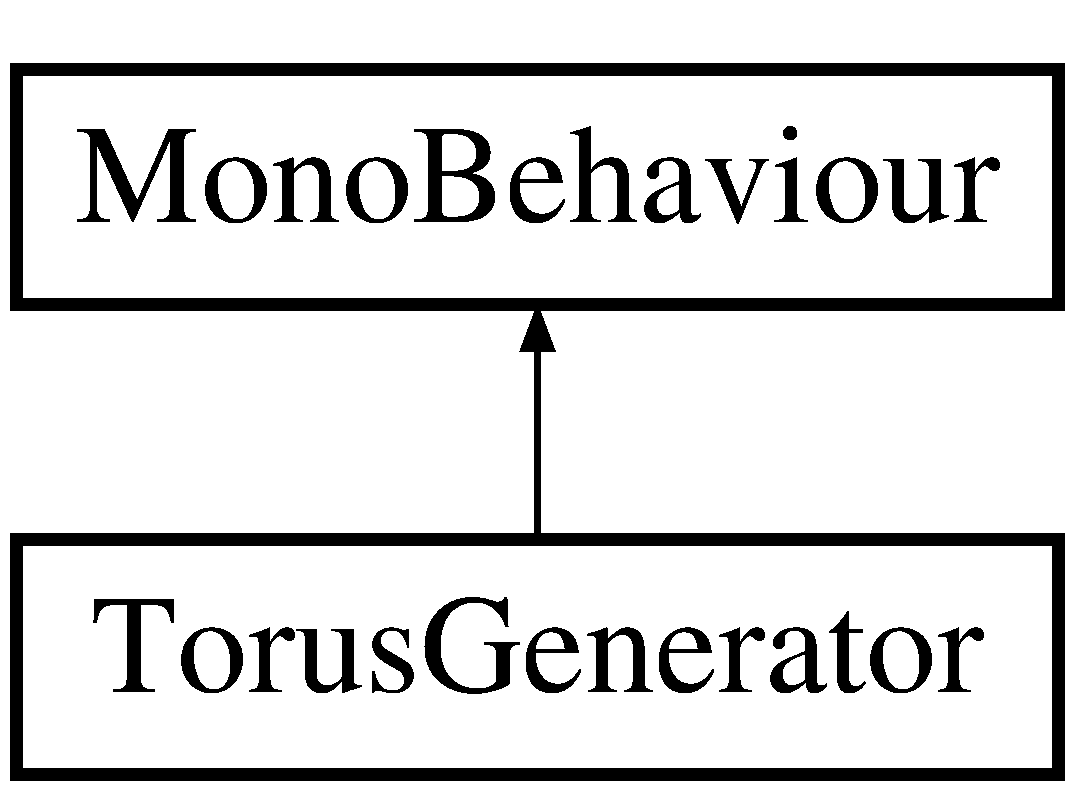
\includegraphics[height=2.000000cm]{class_torus_generator}
\end{center}
\end{figure}
\subsection*{Public Member Functions}
\begin{DoxyCompactItemize}
\item 
void {\bfseries torus} (Game\+Object torus\+Mesh, float segment\+Radius, float tube\+Radius, int num\+Segments, int num\+Tubes)\hypertarget{class_torus_generator_ace97cc7d5209d135b935407b7a554f50}{}\label{class_torus_generator_ace97cc7d5209d135b935407b7a554f50}

\end{DoxyCompactItemize}
\subsection*{Public Attributes}
\begin{DoxyCompactItemize}
\item 
float {\bfseries segment\+Radius} = 1f\hypertarget{class_torus_generator_aed33038eb45157a8feff1e38d07c09bb}{}\label{class_torus_generator_aed33038eb45157a8feff1e38d07c09bb}

\item 
float {\bfseries tube\+Radius} = 0.\+1f\hypertarget{class_torus_generator_a7cbc4daec94ddb0bfbbb2740eb19932c}{}\label{class_torus_generator_a7cbc4daec94ddb0bfbbb2740eb19932c}

\item 
int {\bfseries num\+Segments} = 32\hypertarget{class_torus_generator_ad259d2293d49c58c1ab23418cae7d462}{}\label{class_torus_generator_ad259d2293d49c58c1ab23418cae7d462}

\item 
int {\bfseries num\+Tubes} = 12\hypertarget{class_torus_generator_a7dbdd0f36b47f20ebdf8f235c1d3d27e}{}\label{class_torus_generator_a7dbdd0f36b47f20ebdf8f235c1d3d27e}

\item 
string {\bfseries torus\+Game\+Object\+Name} = \char`\"{}Torus\+Mesh\char`\"{}\hypertarget{class_torus_generator_a0be1daa18ad5c4aa772471ded8e65dbe}{}\label{class_torus_generator_a0be1daa18ad5c4aa772471ded8e65dbe}

\item 
Color {\bfseries color} = Color.\+blue\hypertarget{class_torus_generator_aa8bebfe24d304aa83881e1e676d3fa35}{}\label{class_torus_generator_aa8bebfe24d304aa83881e1e676d3fa35}

\end{DoxyCompactItemize}


The documentation for this class was generated from the following file\+:\begin{DoxyCompactItemize}
\item 
/\+Users/benjamin/\+Programmering/\+Android\+H\+M\+D/\+Tower\+V\+R/\+Assets/\+Scripts/\+Custom/Torus\+Generator.\+cs\end{DoxyCompactItemize}

%--- End generated contents ---

% Index
\backmatter
\newpage
\phantomsection
\clearemptydoublepage
\addcontentsline{toc}{chapter}{Index}
\printindex

\end{document}
